
\begin{figure}[ht]
\begin{Verbatim}[numbers=left,fontsize=\codesize,commandchars=\*\{\}]
type left(node, node).*label{line:language:dict_header1}
type right(node, node).
type linear value(node, int Key, string Value).
type linear replace(node, int Key, string Value).*label{line:language:dict_header2}

replace(A, K, New),*label{line:language:dict_first1}
value(A, K, Old)
   -o value(A, K, New). // we found our key*label{line:language:dict_first2}

replace(A, RKey, RValue),*label{line:language:dict_second1}
value(A, Key, Value),
!left(A, B),
RKey < Key
   -o value(A, Key, Value),
      replace(B, RKey, RValue). // go left*label{line:language:dict_second2}

replace(A, RKey, RValue),*label{line:language:dict_third1}
value(A, Key, Value),
!right(A, B),
RKey > Key
   -o value(A, Key, Value),
      replace(B, RKey, RValue). // go right*label{line:language:dict_third2}

// initial configuration*label{line:language:dict_axioms1}
!left(@0, @1).     !right(@0, @2).
!left(@1, @3).     !right(@1, @4). 
!left(@2, @5).     !right(@2, @6).

value(@0, 3, "a").   value(@1, 1, "b").
value(@2, 5, "c").   value(@3, 0, "d").
value(@4, 2, "e").   value(@5, 4, "f").
value(@6, 6, "g").

// update key 6 to value "x"
replace(@0, 6, "x").*label{line:language:dict_axioms2}
\end{Verbatim}
\caption{LM program for replacing a key's value in a BST dictionary.}
\label{code:language:btree_replace}
\end{figure}

Our second example, shown in Fig.~\ref{code:language:btree_replace}, implements
the key update operation for a binary tree search~(BST) represented as a
key/value dictionary. Each LM node represents a binary tree node. We first
declare all the predicates in
lines~\ref{line:language:dict_header1}-\ref{line:language:dict_header2}.  Linear
predicate \code{value} assigns a key/value pair to a node that can be updated
later. The \code{replace} linear predicate represents an update operation where
the key in the second argument will be updated to the value in the third
argument. As expected, predicates \code{left} and \code{right} represent the
child nodes of each BST node.

The algorithm uses three rules for the three possible cases of updating a key's
value: the first rule
(lines~\ref{line:language:dict_first1}-\ref{line:language:dict_first2}) performs
the update by removing \code{replace(A, K, New)} and \code{value(A, K, Old)}
and deriving \code{value(A, K, New)}; the second rule
(lines~\ref{line:language:dict_second1}-\ref{line:language:dict_second2})
recursively picks the left branch for the update operation by deleting
\code{replace(A, RKey, RValue)} and re-deriving it at node \code{B}; and the
third rule
(lines~\ref{line:language:dict_third1}-\ref{line:language:dict_third2}) picks
the right branch.
The initial facts of this program are presented in
lines~\ref{line:language:dict_axioms1}-\ref{line:language:dict_axioms2} and they
describe the initial binary tree configuration, including keys and values.  The
axiom \code{replace(@0, 6, "x")} instantiated at the root node \code{@3}
manifests the intent to change the value of key 6 to 7.

Figure~\ref{fig:language:btree_trace} represents the trace of the algorithm. The program
database is partitioned by the seven nodes using the first argument of each
fact. In Fig.~\ref{fig:language:btree_trace}~(a), we present the database filled with the
program's initial facts. Next, we follow the right branch using rule 3 since $6
> 3$ (Fig.~\ref{fig:language:btree_trace}~(b)).  We use the same rule again in
Fig.~\ref{fig:language:btree_trace}~(c) where we finally reach the key 6. Here, we apply
rule 1 and \code{value(@6, 6, "g")} is updated to \code{value(@6, 6, "x")}.

\begin{figure}[h]
        \centering
        \begin{subfigure}[b]{0.5\textwidth}
                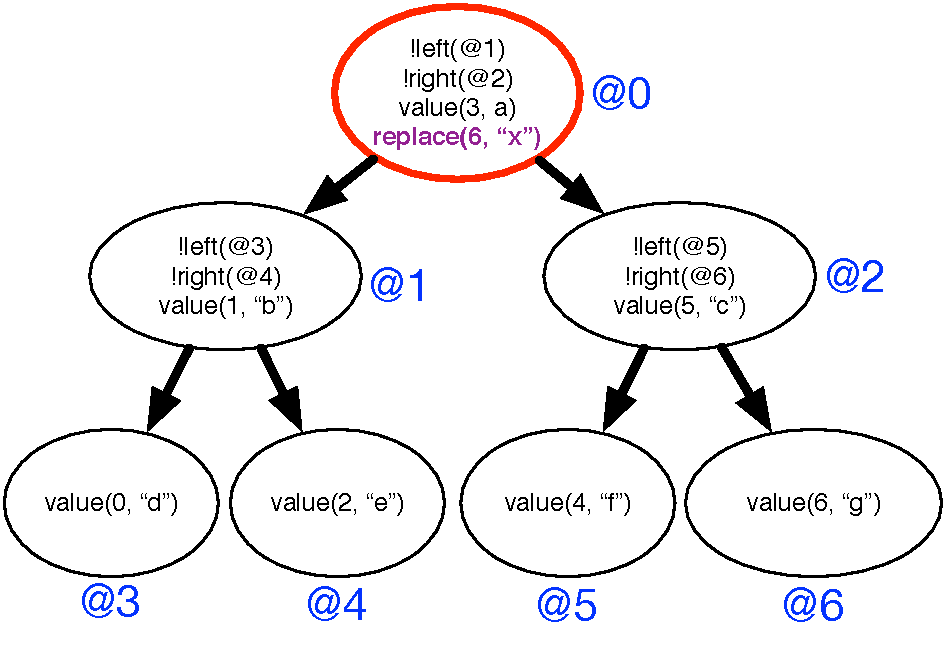
\includegraphics[width=\textwidth]{figures/btree/btree_trace1}
                \caption{Initial database. Replace axiom instantiated at the
                   \code{@3} root node.}
                \label{fig:language:btree_trace1}
        \end{subfigure}%
        ~
        \begin{subfigure}[b]{0.5\textwidth}
                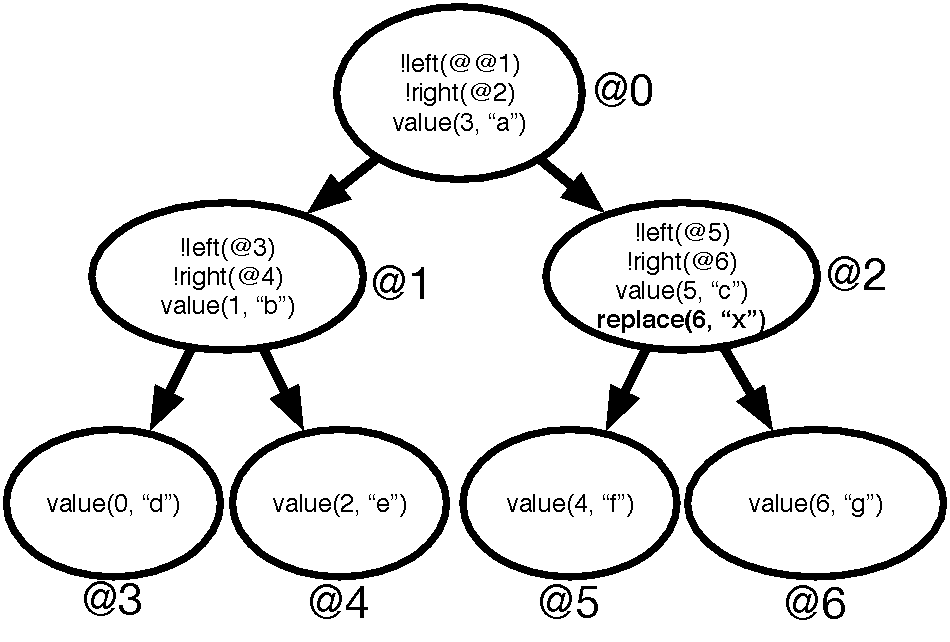
\includegraphics[width=\textwidth]{figures/btree/btree_trace2}

                \caption{After applying rule 3 at node \code{@3}. The
                \code{replace} fact is \emph{sent} (or derived at) to node
                \code{@5}.}

                \label{fig:language:btree_trace2}
        \end{subfigure}\\
        \begin{subfigure}[b]{0.5\textwidth}
                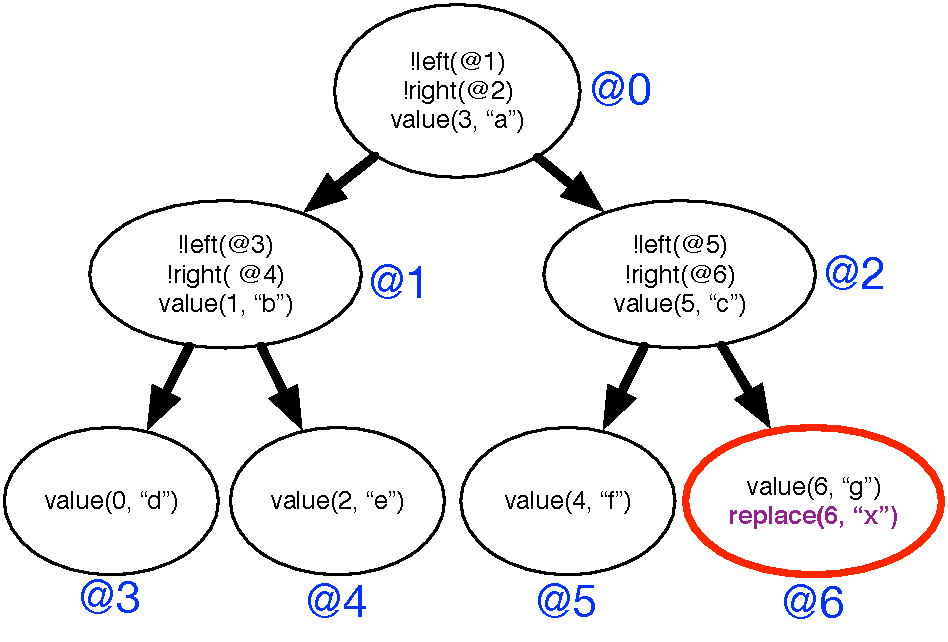
\includegraphics[width=\textwidth]{figures/btree/btree_trace3}
                \caption{After applying rule 3 at node \code{@5}. Replace fact
                   reaches node \code{@6}.}
                \label{fig:language:btree_trace3}
        \end{subfigure}%
        ~
        \begin{subfigure}[b]{0.5\textwidth}
                  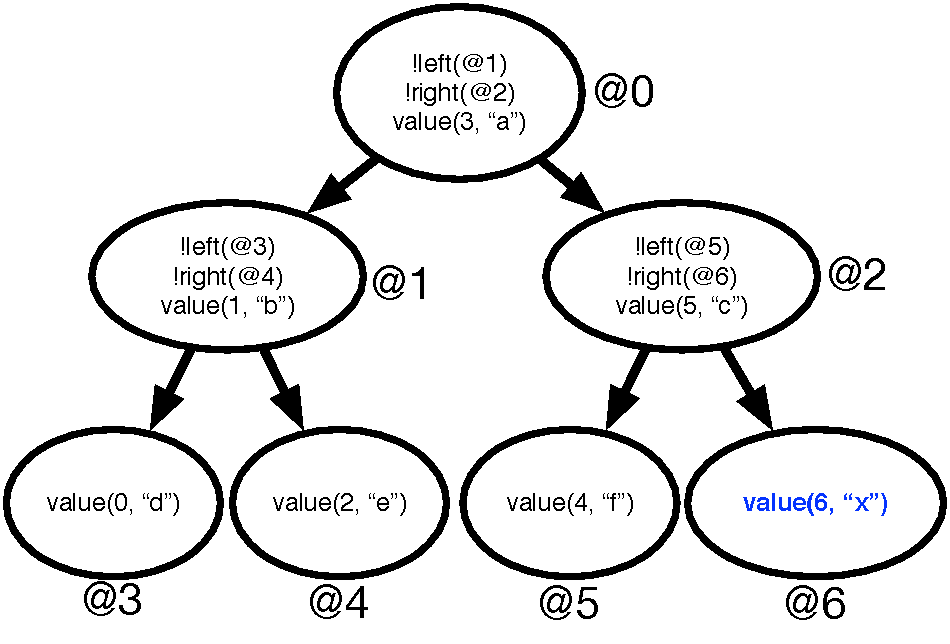
\includegraphics[width=\textwidth]{figures/btree/btree_trace4}
                  \caption{After applying rule 1 at node \code{@6}. Value of key 6 has changed to 7.}
                  \label{fig:language:btree_trace4}
          \end{subfigure}
        \caption{An execution trace for the binary tree dictionary
           algorithm. The first argument of each fact was dropped and the
           address of the node was placed beside it.}\label{fig:language:btree_trace}
\end{figure}

The present example offers many opportunies for concurrency. If we have multiple
\code{replace} facts on different nodes, we can perform multiple value updates
at the same time without introducing any kind of database inconsistency.

